\documentclass[11pt]{article}

\usepackage[utf8]{inputenc}
\usepackage[T1]{fontenc}
\usepackage{lmodern}
\usepackage[margin=1in]{geometry}
\usepackage{amsmath}
\usepackage{amssymb}
\usepackage{graphicx}
\usepackage{booktabs}
\usepackage{caption}
\usepackage[round,authoryear]{natbib}
\usepackage[hidelinks]{hyperref}

\graphicspath{{figures/}}
\captionsetup{font=small,labelfont=bf}
\setlength{\parskip}{0.4em}
\setlength{\parindent}{0pt}

\title{Multi-Sensor Latent-State Fusion for Fundamental Analysis:\\
A Pre-Registered, Point-in-Time Evaluation in Semiconductors}

\author{An\i{}l Berke Karel\\ Politecnico di Torino}

\date{June 2026}

\begin{document}

\maketitle

\begin{abstract}
Does the rhythm of a firm's patenting anticipate its future fundamentals? We frame this as latent-state estimation under noisy observation---borrowing the language of multi-sensor fusion from communications systems---in which a firm's unobserved structural-quality state is sensed through noisy, lagged channels: patent filing rhythm, gross margin, and revenue growth. On a survivorship-aware panel of 52 U.S. semiconductor firms (24 delisted), built entirely from free, reproducible sources (Google Patents on BigQuery and SEC EDGAR XBRL) with full point-in-time reconstruction, we fit a ladder of regime-switching hidden Markov models---a naive count baseline, a single-channel Negative-Binomial model of patent rhythm, and a joint multi-channel fusion model---and evaluate them in a pre-registered, expanding-window, out-of-sample protocol targeting four-quarter-ahead revenue growth. The result is a pre-registered negative: patent-rhythm regime features add no marginal predictive value over simple fundamentals, in any specification and under both a realistic 18-month publication lag and an infeasible oracle, with simple baselines outperforming every model-based feature. Three contributions survive the negative result. First, a diagnosis that naive likelihood-based fusion weights channels by their measurement scale rather than their economic informativeness, confirmed out of sample by a calibration that independently suppresses the count channel to roughly a tenth of its naive weight. Second, a quantification of how restatements inflate momentum backtests---nearly doubling an information coefficient---motivating strict point-in-time discipline. Third, a reproducible evaluation framework, and the argument that count-based patents are the crudest sensor of latent quality: we position quality-weighted, citation-network, and standard-essential-patent signals as the natural next sensors, and provide the harness within which they can be tested honestly.
\end{abstract}

\section{Introduction}

Does the rhythm of a firm's technical activity anticipate its future fundamentals? Innovation is widely held to be a leading indicator of corporate performance, and patents---the most systematically recorded, machine-readable footprint of innovation---are the natural place to test this intuition. A large literature links patent activity to firm value and returns \citep{kogan2017}, and practitioners increasingly market patent-based ``innovation momentum'' signals. Yet most of this work measures patents as a \emph{level}---counting them, perhaps weighted by citations or value---rather than asking whether the \emph{temporal dynamics} of patent production carry forward-looking information about fundamentals.

This distinction matters because counting conflates two very different firms: a structurally ascending company whose accelerating patent output reflects a genuine expansion of its technological frontier, and a deeply cyclical one whose output rises simply because the whole industry is in an up-cycle. Counted naively, both look identical---patents are rising. To be useful, a method must separate the structural signal from the cyclical noise, and do so \emph{ex ante}, using only information available at decision time.

We frame this as latent-state estimation under noisy observation, borrowing the language of multi-sensor fusion from communications and tracking systems. A firm's unobserved ``structural quality state'' cannot be measured directly; instead, each data channel---patent filing rhythm, gross margin, revenue growth---acts as a noisy, lagged, intermittently observed sensor of that hidden state. The natural model is a regime-switching state-space system: the hidden state follows a Markov chain, and the channels are conditionally independent emissions. This is, in a precise sense, the same mathematics used to track a latent channel state from noisy received symbols in a communications receiver, applied here to a latent quality state. The central question becomes whether \emph{fusing} channels recovers a signal that no single channel---least of all naive patent counts---provides alone.

Answering this credibly demands discipline on three fronts that prior work often treats lightly: \textbf{point-in-time} information (patent applications are secret for $\sim$18 months, and financials are released and frequently restated long after the quarter they describe, so naive series leak future information); \textbf{survivorship} (a heavily consolidated industry requires the acquired and delisted firms that a currently-listed universe omits); and \textbf{pre-registration} (with many candidate signals, horizons, and model variants, we fix feature sets, windows, targets, and metrics in advance and report every result against them, with a deviation log).

We assemble a survivorship-aware panel of 52 U.S. semiconductor firms (24 delisted) from two reproducible, no-cost sources---Google Patents Public Data on BigQuery for harmonized patent records with three event dates, and SEC EDGAR XBRL for point-in-time quarterly fundamentals---spanning 2009--2023. On it we build a ladder of models---a naive count baseline, a single-channel Negative-Binomial hidden Markov model of patent rhythm, and a joint multi-channel fusion model---and evaluate each in a pre-registered, expanding-window out-of-sample protocol targeting four-quarter-ahead revenue growth, against deliberately simple baselines.

Our headline result is negative, and we report it as such: in this universe and period, patent-rhythm regime features add no marginal predictive value for future revenue growth over simple fundamentals---whether the patent channel is used alone, in naive fusion, or in calibrated fusion, and whether under a realistic 18-month publication lag or an infeasible oracle. Simple baselines outperform every hidden-Markov feature, though all signals are weak, indicating the target itself is only marginally predictable here.

Our contribution is therefore not a profitable signal but a method and a disciplined verdict: (i) a reproducible, survivorship-aware, point-in-time fusion framework for evaluating technical and financial signals against fundamentals, built entirely on free data; (ii) two data-discipline findings independent of the predictive result---a measurement of how restatements inflate momentum backtests, and a characterization of the structural filing-to-grant lag; (iii) a diagnosis that naive likelihood-based fusion weights channels by measurement scale rather than economic informativeness, with out-of-sample confirmation that data-driven calibration suppresses the dominant channel to $\sim$10\% weight; and (iv) a pre-registered negative result, reported with its full deviation log. We position count-based patents as the crudest possible sensor and identify quality-weighted, citation-network, and standard-essential-patent signals as the natural next sensors to fuse.

\section{Related Work}

Our work sits at the intersection of four literatures, and its contribution is defined by a gap none of them fills.

\textbf{Patents and firm value.} A large body of work establishes that patents carry economic information. \citet{kogan2017} measure the value of individual patents from stock-price reactions to their grants and link these estimates to subsequent growth and reallocation; a wide literature relates patent counts and citations to returns, productivity, and valuation. This work overwhelmingly treats patents as a \emph{level}---a stock, possibly quality-weighted---and targets stock returns. We differ on both axes: we study the \emph{temporal dynamics} of patent production rather than its level, and we target \emph{fundamentals} (revenue growth) rather than returns, a less-crowded and arguably more structural question.

\textbf{Regime-switching and state-space models in finance.} Markov regime-switching models have been standard in financial econometrics since \citet{hamilton1989}, used to capture latent states such as recessions and expansions, and state-space methods underpin much of nowcasting and mixed-frequency estimation, where series observed at different frequencies are combined to track a latent state. We adopt this machinery but apply it to an unusual observation set---fusing a count-valued technical channel with continuous financial channels---and our scale diagnosis is, in effect, a caution about applying it naively to heterogeneous sensors.

\textbf{Machine learning for fundamentals.} A growing literature forecasts corporate fundamentals with machine learning. \citet{chen2022} predict the direction of one-year-ahead earnings changes from high-dimensional financial data with significant out-of-sample power, and \citet{cao2024} find machine-learning earnings forecasts that outperform both extant models and analyst consensus. This work establishes both the target (forward fundamentals) and the methodological standard (rolling-window estimation, cross-validated, designed to avoid look-ahead) that we adopt. Our addition is a \emph{technical} channel alongside the financial features these studies use, evaluated under the same out-of-sample discipline.

\textbf{Point-in-time discipline and reproducibility.} A recurring theme in the real-time forecasting literature is that backtests using as-currently-reported data overstate performance, because the data a researcher downloads today differs from what was knowable in the past. We take this concern to its logical conclusion: we reconstruct both patent and financial channels at their point-in-time state, retain filing timestamps on every financial fact, separate as-filed from restated series, and---departing from common practice---pre-register the entire predictive evaluation. To our knowledge, no prior study combines a patent-rhythm signal, a fundamental target, full point-in-time reconstruction, and pre-registration; that combination is this paper's methodological contribution, independent of its negative empirical verdict.

\section{Data and Point-in-Time Discipline}

We construct our panel from two public, no-cost, reproducible sources: Google Patents Public Data, accessed via BigQuery, for patent records, and the U.S. Securities and Exchange Commission's EDGAR XBRL API for financial statements. Both choices are deliberate: the data are free, the queries are reproducible from the replication materials, and---critically for our research question---both expose the dates required to reconstruct what was knowable at any past decision point.

\subsection{Patent data and assignee resolution}

The \texttt{patents-public-data.patents.publications} table provides, for each publication, three integer event dates---filing, publication, and grant---together with a harmonized assignee field that consolidates name variants under a standardized entity name. Harmonization resolves the bulk of the entity-matching problem that complicates patent research: for example, a single firm's filings under ``NVIDIA Corp,'' ``Nvidia Corporation,'' and assorted misspellings collapse to one assignee. We match firms to assignees by prefix on the harmonized name, which we found preferable to substring matching: a substring rule on ``NVIDIA'' admits false positives such as ``INVIDIATO COSMO'' and ``CONVIDIA WIRELESS,'' whereas a prefix rule does not.

Harmonization is necessary but not sufficient, and two failure modes required explicit handling. First, the harmonized field occasionally abbreviates a firm's name in a way that breaks a naive full-name match: a prefix derived from ``National Semiconductor'' returns nothing, because the harmonized entity is ``NAT SEMICONDUCTOR'' (4,979 filings). A low-count alarm---flagging any expected-large firm whose match returns implausibly few patents---caught six such cases that would otherwise have been silently emptied. Second, the prefix rule itself admits a small tail of genuine false positives (different companies and individuals' names sharing a prefix) and legitimate subsidiaries; we resolve these with a symmetric rule applied identically across all firms, documented in the replication materials: assignees verifiably belonging to a different company or to an individual are excluded; names with at least twenty filings are verified individually, and ambiguous names below ten filings are retained as documented residual noise. A patent is collapsed to a single application via its application number, merging the pre-grant (A-document) and granted (B-document) records that the publications table stores as separate rows, so that each application is counted once.

\subsection{Financial data and point-in-time reconstruction}

For each firm we retrieve quarterly fundamentals from a single EDGAR \texttt{companyfacts} call, extracting revenue, cost of revenue (for gross margin), and operating income. Three issues of XBRL practice required care. First, \textbf{tag variants}: the concept for revenue is reported under different us-gaap tags across firms and over time---\texttt{Revenues}, \texttt{Revenue\allowbreak From\allowbreak Contract\allowbreak With\allowbreak Customer\allowbreak Excluding\allowbreak Assessed\allowbreak Tax}, \texttt{SalesRevenueNet}, and others---and the transition to the ASC 606 revenue standard around 2018 induces a tag change for most firms. We resolve revenue by trying a priority-ordered list of tags and log, per firm, which tag covered which span; one firm (AMD) reported 2009--2015 revenue only under \texttt{SalesRevenueGoodsNet}, a tag that would have left it revenue-less before 2012 had it not been added. Second, \textbf{Q4 derivation}: 10-K filings report full-year figures, so the fourth fiscal quarter of a flow variable is not reported directly and must be derived as FY minus the sum of Q1--Q3; we always derive Q4 this way for a uniform information timestamp (the 10-K date) and use any directly-reported Q4 facts only as a cross-check, because some are first published only in a comparative filing one to two years later.

Third, and most important for our question, is the \textbf{fiscal-calendar mismatch}: three of our four case-study firms do not close their fiscal year in December---NVIDIA and Marvell close in late January, Micron in late August---so a label such as ``NVIDIA FY2024 Q4'' actually falls in calendar Q4 2023. We therefore align every observation to a calendar quarter by its XBRL period-end date, not by its fiscal-year/period label; aligning by label would shift the affected series by roughly a year and silently corrupt every cross-channel comparison. For point-in-time correctness, we retain the \texttt{filed} date on every fact as the timestamp at which the figure became public knowledge. Where a quarter is restated---the same period reported with different values in later filings---we keep the earliest-filed value as the \emph{as-filed} series (used in all point-in-time analysis) and the most recent value as a separate \emph{latest} series; the two differ for a non-trivial number of observations and, as Section~3.4 shows, the choice between them is consequential.

\subsection{Universe construction: survivorship and entity continuity}

Our universe is defined by a pre-registered rule, with every inclusion and exclusion documented. We begin with all 10-K filers under SIC code 3674 (Semiconductors and Related Devices), including delisted firms, which EDGAR retains after delisting; we require at least \$500M in annual revenue at some point during 2009--2023 (using the union of revenue tag variants) and at least eight quarters of XBRL depth. A device-category screen removes solar/PV, equipment and materials, optical-module, and foreign (20-F filing) firms, each set documented with its rationale. Because the rule as written excludes Qualcomm---filed under SIC 3663---we add it back via a documented amendment, with the decision stamped into the registry before any predictive analysis was run. The result is 52 firms, of which 24 are delisted. Retaining delisted firms is the central survivorship safeguard and a concrete advantage of the free-SEC route over convenience data sources that drop delisted tickers; acquired companies such as Xilinx, Altera, Cypress, and Inphi enter the panel over their own historical windows, with no forward-filling.

Consolidation also threatens \emph{entity continuity} in two ways that we flag and handle. First, the SEC ticker map may point only to a post-merger legal entity: Marvell's map returned only the entity created in the 2021 Inphi combination, so we add the predecessor CIK and merge the two over their respective periods. Second, mergers reattribute innovation: when one firm acquires another, post-close filings under the acquired firm's name represent the acquirer's activity. We apply a reattribution rule that splits patent attribution at the deal close date, with no double-counting between in-universe firms, supported by a documented table of major transactions. This rule moves, for example, post-2020 Mellanox filings to NVIDIA and post-2022 Xilinx filings to AMD, and drops series flowing to out-of-universe acquirers.

\subsection{Two data-discipline findings}

The reconstruction above is not merely bookkeeping; it surfaces two findings that hold independently of any predictive result.

\textbf{The filing-to-grant lag is substantial and varies across firms.} Across our case-study firms the mean filing-to-grant lag ranges from roughly 28 to 43 months and is not constant (coefficient of variation $\approx 0.20$): grants are slowest for NVIDIA ($\sim$43 months mean) and fastest for Micron ($\sim$28 months). The filing-to-publication lag clusters near the textbook eighteen months for some firms but shows an anomalous shorter mode for others. The practical implication is direct: a signal built on grant dates dates innovation two to three years late, and even a filing-date signal is unobservable in real time for roughly the first eighteen months after filing---a constraint we make explicit in the predictive evaluation rather than assume away (Figure~\ref{fig:lag}).

\begin{figure}[htbp]
  \centering
  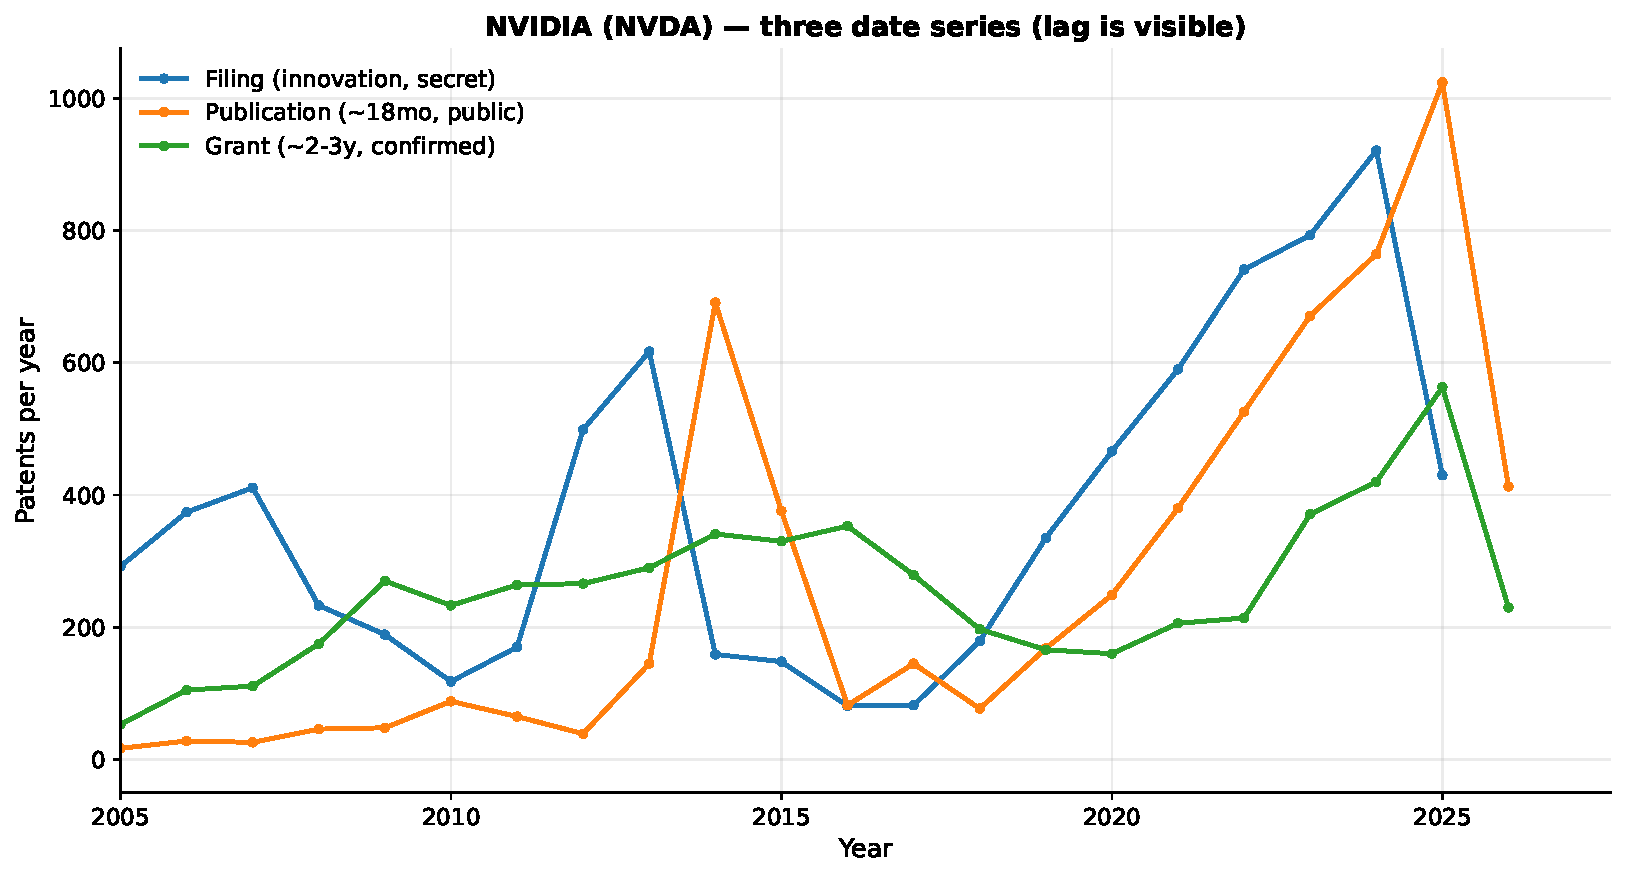
\includegraphics[width=0.82\linewidth]{fig01_lag.pdf}
  \caption{\textbf{The filing-to-grant lag, illustrated for NVIDIA.} NVIDIA's patent activity dated by the three event dates the publications table exposes---filing, publication, and grant (yearly counts). The horizontal displacement between the curves is the lag: a grant-dated signal trails the underlying filing activity by two to three years, and even a filing-dated signal is invisible for roughly the first eighteen months after filing. The cross-firm variation in mean lag ($\approx$28--43 months, CV $\approx$ 0.20) is reported in the text.}
  \label{fig:lag}
\end{figure}

\textbf{Restatements inflate momentum backtests.} Because we retain both as-filed and latest financial series, we can quantify the cost of the common practice of backtesting on restated data. A simple revenue-momentum signal---itself one of our baselines---earns an information coefficient of $+0.039$ against the as-filed target but $+0.079$ against the latest (restated) target, roughly doubling its apparent strength. The mechanism is that restatements tend to align, in hindsight, with the direction the signal was already pointing; using point-in-time as-filed data removes this look-ahead and prevents the signal from appearing stronger than it was knowable to be. In our setting this is a concrete, quantified caution against backtesting fundamental signals on as-currently-reported data; while we measure it on a single signal in one industry, the mechanism---restatements aligning in hindsight with the signal---is general, and we expect it to operate wherever point-in-time data is not used (Figure~\ref{fig:restate}).

\begin{figure}[htbp]
  \centering
  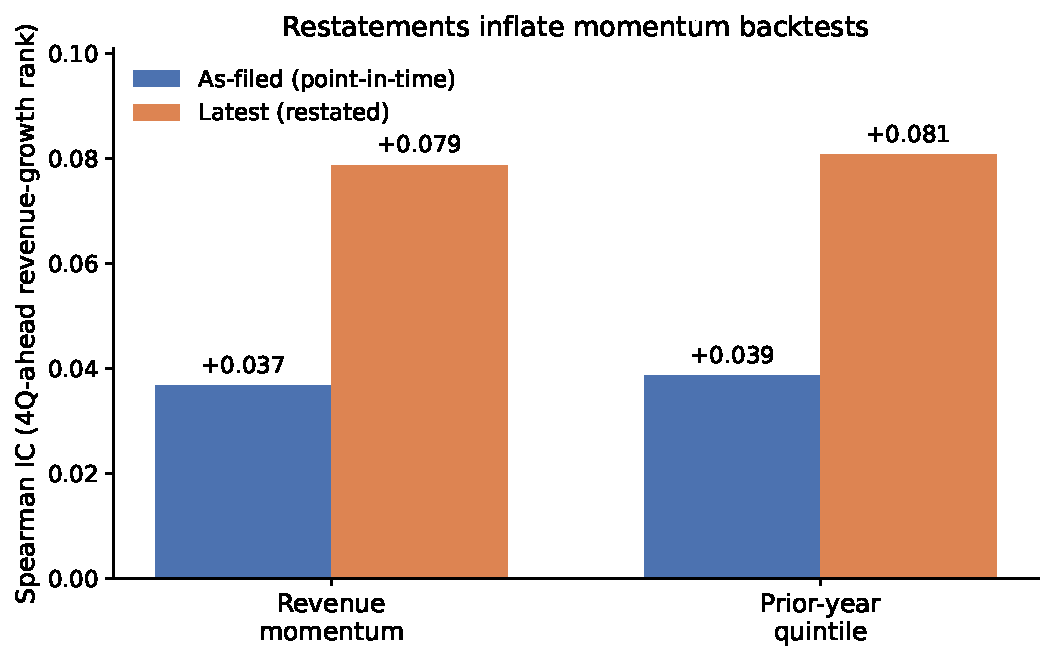
\includegraphics[width=0.7\linewidth]{fig02_restatement.pdf}
  \caption{\textbf{Restatements inflate momentum backtests.} The same momentum baselines scored against the as-filed (point-in-time) target versus the most-recently-restated (latest) target. Each signal's information coefficient roughly doubles on restated data---look-ahead introduced by restatements aligning, in hindsight, with the direction the signal already pointed.}
  \label{fig:restate}
\end{figure}

\section{Single-Channel Regime Models}

Before fusing channels, we establish what a single channel---patent rhythm alone---can and cannot reveal. This serves two purposes: it provides the naive and single-channel baselines against which fusion is later measured, and it establishes, at the model level, the central motivation for fusion.

\subsection{Model specification}

We model each firm's quarterly patent-filing count as the emission of a two-state hidden Markov model, where the latent state represents a low or high innovation-tempo regime. We use a Negative-Binomial emission rather than Poisson because patent counts are strongly overdispersed---their variance far exceeds their mean---and a Poisson emission, which assumes equality, is misspecified. The model has, per state, a state-dependent mean (constrained so that state 0 is the low-tempo and state 1 the high-tempo regime), a shared dispersion parameter, a two-by-two transition matrix, and an initial distribution. We fit each firm independently; pooling across firms is deferred to the panel evaluation. We restrict the analysis to complete quarters: the most recent $\sim$18 months of filing data are incomplete by construction---filed applications remain unpublished and thus invisible---and including them would manufacture a spurious low-tempo regime, so we truncate at the last fully-observed quarter and stamp the truncation date on every output.

\subsection{Estimation and validation}

We estimate parameters by Expectation-Maximization. Because a reliable Negative-Binomial HMM was not available off the shelf, we implement the forward-backward recursion in log-space (using the log-sum-exp identity) to guard against numerical underflow, with the dispersion parameter optimized numerically within each M-step. We run twenty random restarts per firm and retain the highest-likelihood solution, reporting the stability of the restarts. After fitting, states are ordered by their emission mean so that ``high regime'' is comparable across firms---without this label-ordering step, cross-firm comparison would be meaningless.

We validate the implementation in two ways consistent with the synthetic-verification discipline we apply throughout. First, on short synthetic sequences we confirm that the log-space forward-backward agrees with a brute-force enumeration of all state paths to a precision of $10^{-10}$. Second, on synthetic data generated from a known Negative-Binomial HMM, we confirm that EM recovers the true parameters (means within $\pm$15\%, transition diagonal within $\pm$0.05, state-classification accuracy $\approx$98\%). The Negative-Binomial specification is decisively preferred over Poisson on the real data, improving BIC by between 204 and 1,092 across firms.

\subsection{Results: persistence distinguishes, but only in hindsight}

We report regime estimates for four case-study firms chosen to span the relevant variation: NVIDIA (a firm that experienced a large revenue expansion), AMD (a cyclical recovery), Marvell (a mid-cap networking firm), and Micron (an extreme memory cycle, included deliberately as a control whose revenue is driven by supply-demand dynamics rather than by patent activity). For each firm the model yields filtered (causal) and smoothed (full-sample) regime probabilities; we report the filtered switch dates, defined as persistent crossings of probability 0.5 sustained for at least two quarters (Figures~\ref{fig:reg-nvda}--\ref{fig:reg-mu}).

\begin{figure}[htbp]
  \centering
  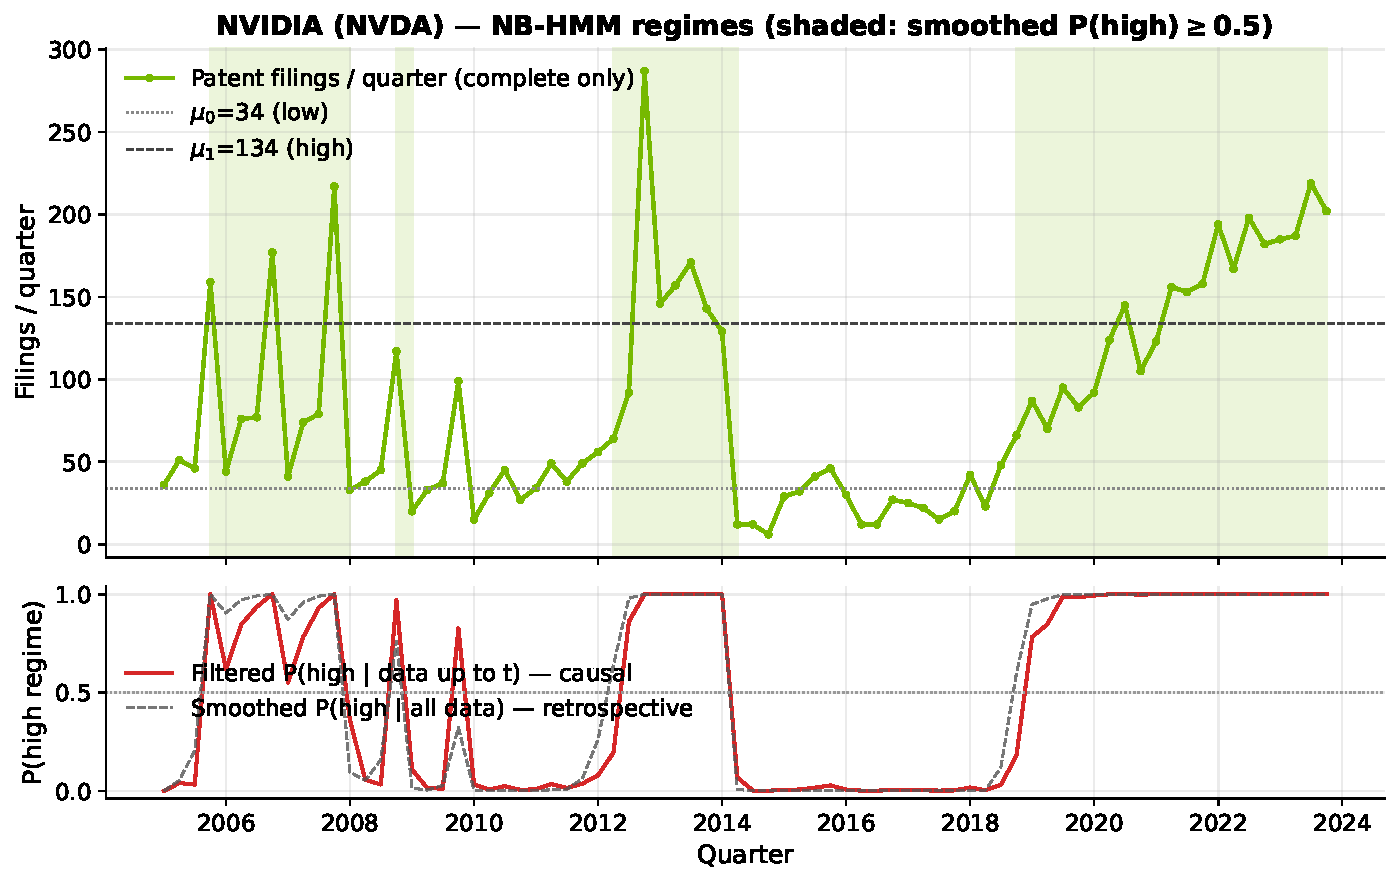
\includegraphics[width=0.92\linewidth]{fig03_regime_nvda.pdf}
  \caption{\textbf{NVIDIA --- NB-HMM patent-rhythm regimes.} Quarterly filing counts with smoothed high-regime periods shaded (upper panel) and the filtered (causal) versus smoothed high-regime probability (lower panel). NVIDIA enters a high-tempo regime in 2019Q1 and does not leave it through the end of the sample.}
  \label{fig:reg-nvda}
\end{figure}

\begin{figure}[htbp]
  \centering
  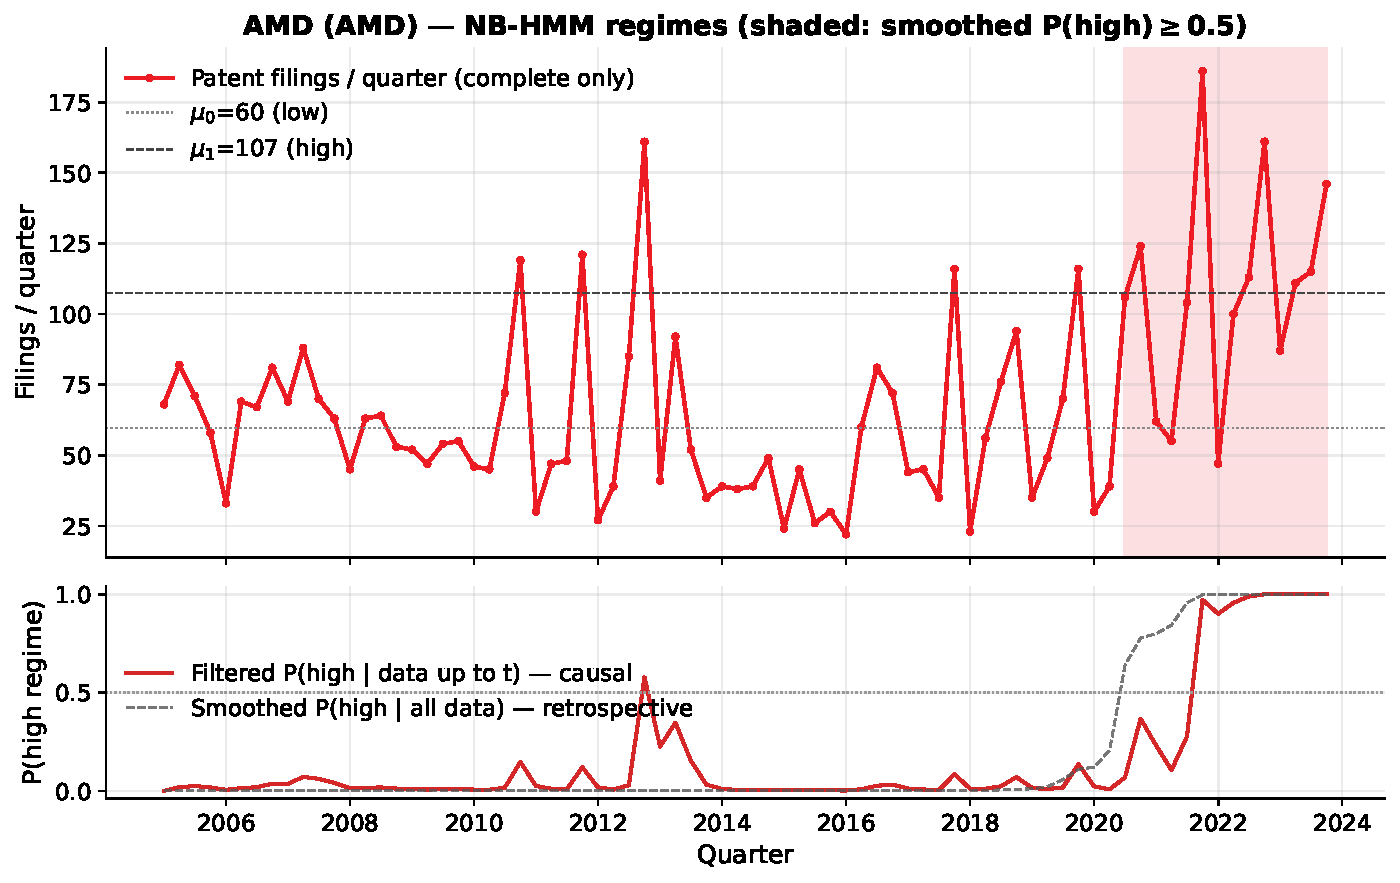
\includegraphics[width=0.92\linewidth]{fig04_regime_amd.pdf}
  \caption{\textbf{AMD --- NB-HMM patent-rhythm regimes.} As Figure~\ref{fig:reg-nvda}. AMD's patent separation is weak (a high-to-low mean ratio of only $\sim$1.5), so its regime structure is less sharply defined.}
  \label{fig:reg-amd}
\end{figure}

\begin{figure}[htbp]
  \centering
  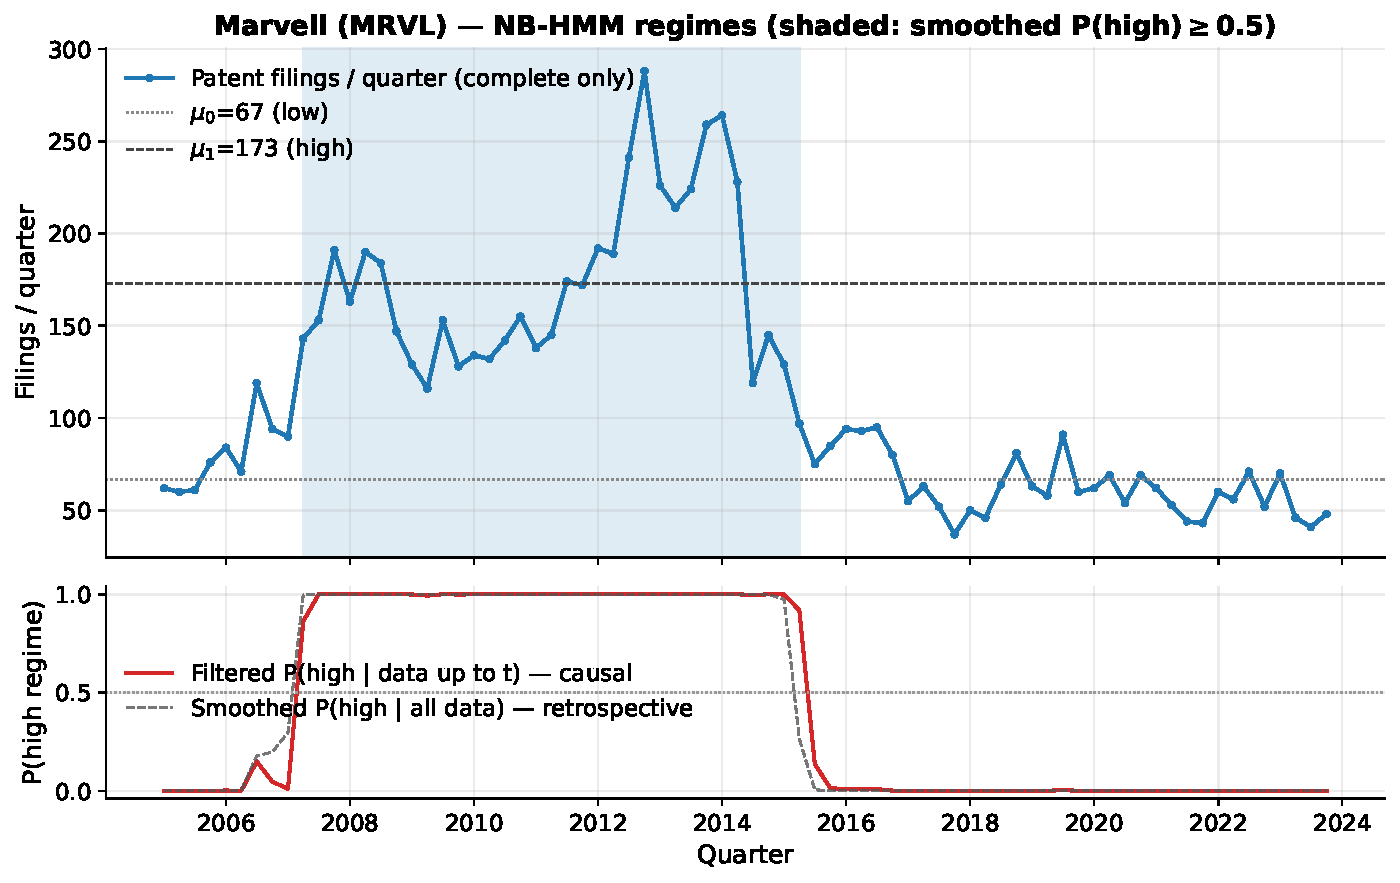
\includegraphics[width=0.92\linewidth]{fig05_regime_mrvl.pdf}
  \caption{\textbf{Marvell --- NB-HMM patent-rhythm regimes.} As Figure~\ref{fig:reg-nvda}, for a mid-cap networking firm.}
  \label{fig:reg-mrvl}
\end{figure}

\begin{figure}[htbp]
  \centering
  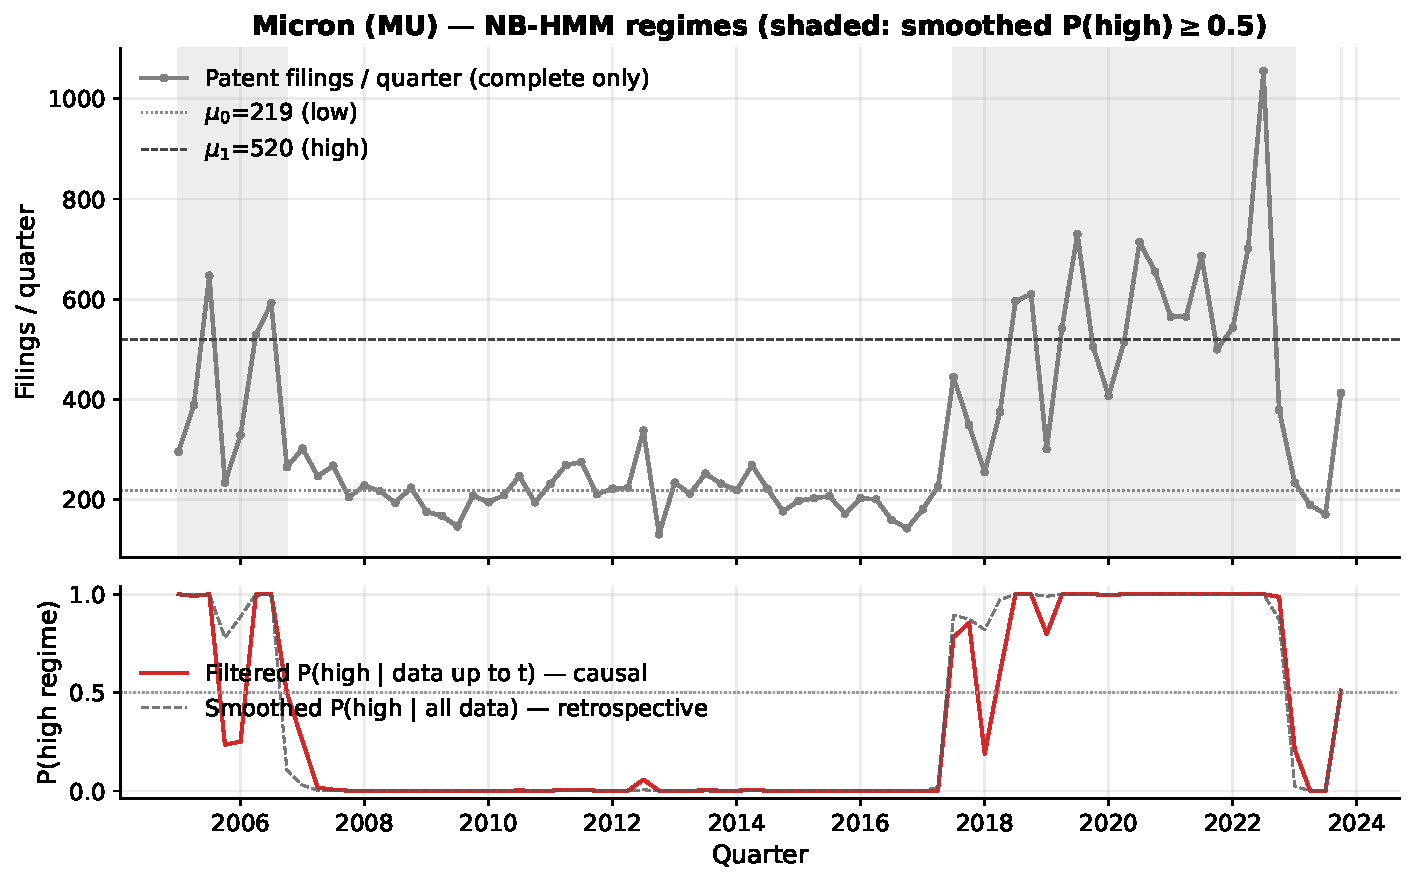
\includegraphics[width=0.92\linewidth]{fig06_regime_mu.pdf}
  \caption{\textbf{Micron --- NB-HMM patent-rhythm regimes.} As Figure~\ref{fig:reg-nvda}, for the memory-cycle control. Micron enters a high-tempo regime in 2017Q3---earlier than NVIDIA---and exits in 2023Q1 as the memory cycle turns; the patent channel cannot foresee the subsequent revenue collapse.}
  \label{fig:reg-mu}
\end{figure}

The central finding is that a single channel cannot separate structural signal from cyclical noise \emph{ex ante}. NVIDIA enters a high-tempo regime in 2019Q1 and does not leave it through the end of the sample, with a high-to-low mean ratio of roughly four---consistent with a structural ascent preceding its revenue expansion. But the control firm switches too: Micron enters a high-tempo regime in 2017Q3---\emph{earlier} than NVIDIA---and exits in 2023Q1 as the memory cycle turns. An investor following a patent-rhythm regime signal in 2017 would thus have received a ``structural ascent'' indication from Micron, whose subsequent revenue collapse the signal could not foresee. The two firms can be distinguished only in their persistence---NVIDIA never exits, Micron exits with the cycle---but this is a hindsight distinction: at the moment of the Micron signal, both firms appeared identically to be in a sustained high regime. The information needed to tell them apart in real time is not in the patent channel. This is the motivation for fusion, made precise.

\section{Naive Fusion and the Scale Problem}

We now fuse channels. The single-channel analysis identified the information needed to separate structural from cyclical regimes as residing outside the patent channel; the natural hypothesis is that financial channels supply it, and that a joint model recovers a latent state that neither channel reveals alone.

\subsection{Joint model specification}

We extend the hidden Markov model so that a single latent state emits three conditionally-independent channels: patent count (Negative-Binomial, as before), gross margin (Gaussian), and revenue growth (Gaussian). The quarterly log-emission is the sum of the log-densities of the channels observed that quarter. Missing channels are handled natively by omitting their term---the financial channels are unavailable before 2009 while the patent channel extends earlier---which is the same mechanism that lets a state-space filter track through intermittent sensor dropouts, and which we prefer to imputation. We retain the estimation machinery of Section~4 (log-space EM, twenty restarts, label-ordering), adding a variance floor on the Gaussian channels to prevent a state from collapsing onto a single observation, and we verify on synthetic three-channel data, including with masked channels, that EM recovers the true parameters.

\subsection{A pre-registered separation test, and its failure}

We registered a specific test before estimation: if fusion supplies the missing information, the joint model's filtered probability should exit Micron's high regime \emph{early}---as the memory cycle's margin collapse arrives around 2019---rather than persisting to 2023 as the patent-only model did. The test is pre-specified precisely so that a result either way is informative, and so that we cannot tune the model toward the outcome we want.

The hypothesis was not supported. In the joint model, Micron exits the high regime at the same date as the patent-only model (2023Q1), not in 2019; through the 2019 margin collapse its filtered high-regime probability remains above 0.96. Fusion did not, as specified, rescue the separation. We report this as the registered result, without adjustment (Figure~\ref{fig:fusion}).

\begin{figure}[htbp]
  \centering
  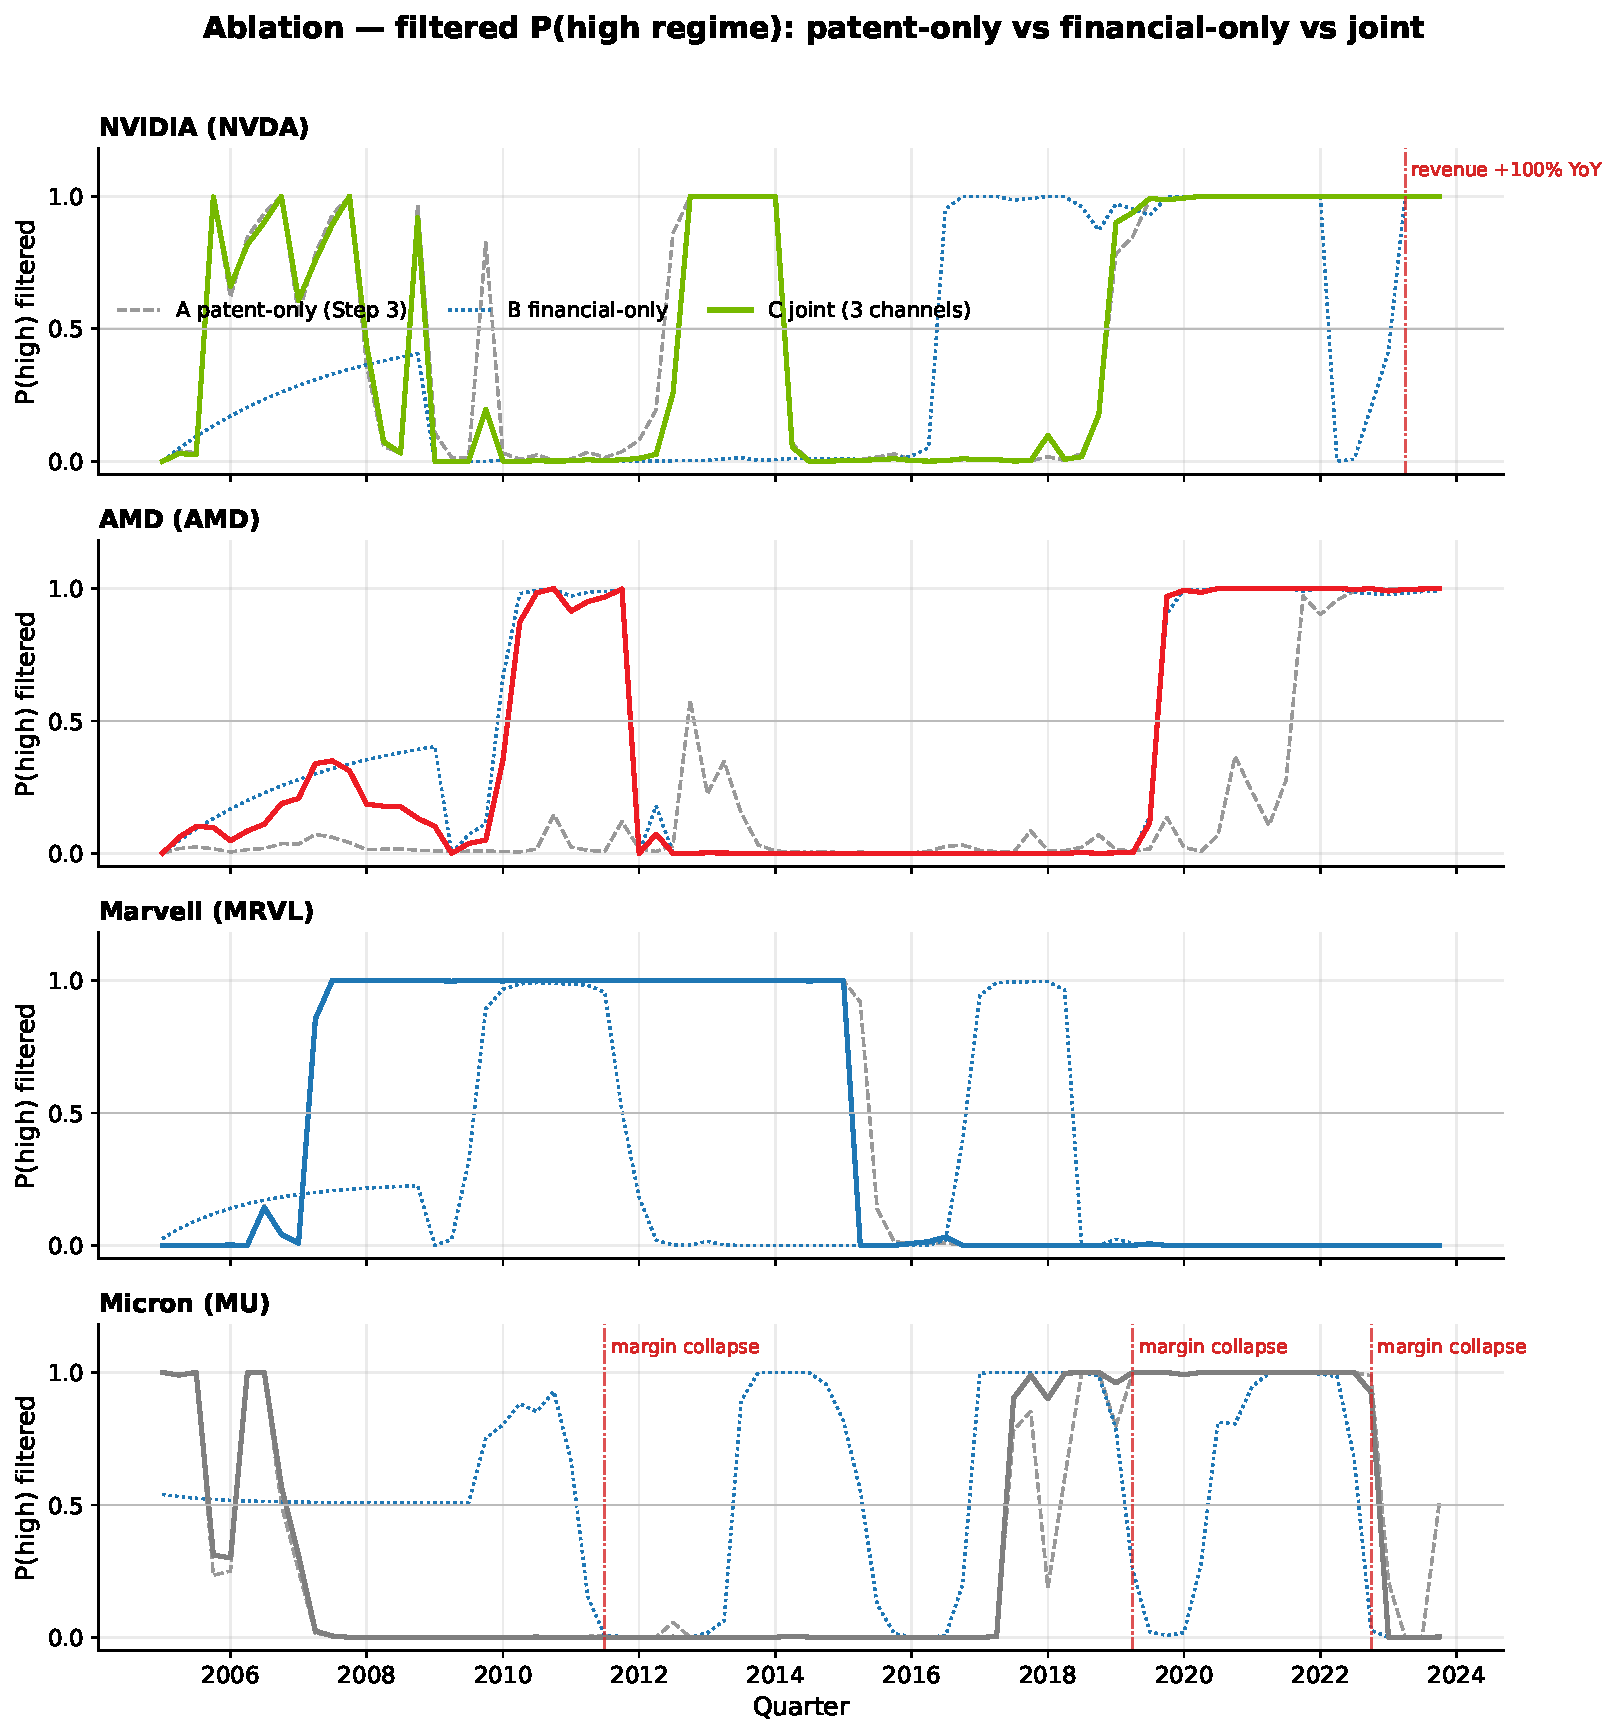
\includegraphics[width=0.92\linewidth]{fig07_fusion.pdf}
  \caption{\textbf{The pre-registered separation test fails.} Filtered high-regime probability for the patent-only, financial-only, and joint (three-channel) models, with data-derived event markers. The joint model's regime exits are far sharper and more robust at the sample edge, but it does not exit Micron's high regime early as the registered hypothesis required.}
  \label{fig:fusion}
\end{figure}

Fusion is not, however, without effect, and the effects are instructive. The joint model's regime \emph{exits} are far sharper---at the 2023Q1 exit its high-regime probability is on the order of $10^{-8}$ versus 0.21 for the patent-only model---and it is more robust at the sample edge: a late surge of filings drives the patent-only probability back up to 0.51 (``Micron is high again''), while the joint model, lacking financial confirmation, stays near 0.002. A financial-only variant cleanly dates the memory cycle on its own (high in 2020Q3, low in 2022Q4) and reveals a short high-margin window for Marvell around the Cavium acquisition that no patent-bearing model detects. The channels carry distinct information; the failure is in how the naive joint model combines it.

\subsection{Diagnosis: implicit weighting by measurement scale}

The failure has a precise mechanical cause. Under conditional independence, each channel contributes to the posterior in proportion to its own log-likelihood, and the Negative-Binomial log-likelihood of a count on the order of five hundred per quarter is far larger in magnitude---and far more discriminating between its own states---than the Gaussian log-likelihood of a single quarter's margin or growth. The joint model therefore weights channels by their \emph{measurement scale and statistical separability, not by their economic informativeness about the latent quality state}. The patent channel's high statistical precision about its own mean does not imply high information about future fundamentals; under misspecification, the likelihood overstates that precision, and the count term dominates. AMD displays the mirror image: there the patent separation is weak (a high-to-low mean ratio of only 1.5), the Gaussian channels win, and the model effectively becomes the financial-only narrative---so what the joint model ``believes'' varies arbitrarily across firms with the scale of the count, not with signal quality.

This diagnosis reframes the question. The problem is not whether to fuse but \emph{how}: a principled fusion must weight channels by their predictive contribution rather than their nominal likelihood. We do not solve this by ad hoc rescaling here; instead we let the out-of-sample evaluation of Section~6 determine channel weights by their actual predictive value, which both tests the diagnosis and provides the calibrated competitor (Figure~\ref{fig:state}).

\begin{figure}[htbp]
  \centering
  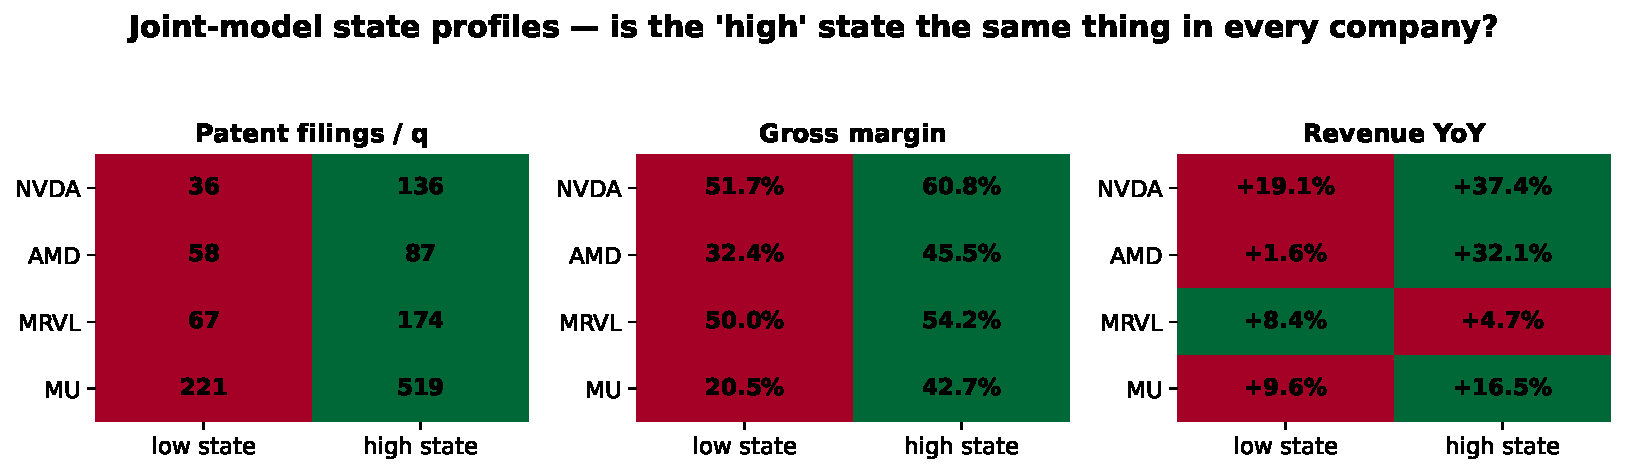
\includegraphics[width=0.92\linewidth]{fig08_state_means.pdf}
  \caption{\textbf{Joint-model state-conditional channel means.} For each case-study firm, the low- and high-state means of the three channels (patent count, gross margin, revenue growth). Color is scaled within company so the low$\to$high direction is visible: a high-patent state whose financial cells run the other way marks a firm where patents and financials disagree, illustrating that ``high'' does not mean the same thing everywhere.}
  \label{fig:state}
\end{figure}

\section{Pre-Registered Predictive Evaluation}

The descriptive analysis showed that naive fusion mis-weights channels; the predictive question---whether patent-rhythm regime features add value over simple fundamentals when weights are set by predictive performance---can only be answered out of sample. We pre-register the entire evaluation: feature sets, candidate models, prediction dates, targets, metrics, and baselines are fixed in advance, and we report every result against them, including a deviation log (Appendix~B). The discipline is the point: with this many moving parts, a selectively-reported positive would be uninformative.

\subsection{Protocol}

The primary target is four-quarter-ahead revenue growth, expressed as a within-universe rank at each prediction date, scored by the cross-sectional Spearman information coefficient (IC) with Newey-West-corrected significance; an eight-quarter horizon is evaluated as a secondary target. All targets are built from the as-filed series, so that both predictors and outcomes respect the information available in real time. Firms remain in the panel only while they are alive; a firm delisted within the horizon yields no target and drops out, and we report the resulting attrition explicitly.

Two disciplines govern what the patent channel may know at prediction time $t$. We evaluate it in two variants: a \emph{feasible} series, truncated at $t-6$ quarters to respect the $\sim$18-month publication lag, so that only genuinely-visible filings inform the prediction; and an \emph{oracle} series, using filings up to $t$, which is infeasible in real time and serves only as an upper bound. The difference between them is our numerical answer to whether the publication lag costs predictive information. The financial channel uses only observations with a filed date on or before $t$. Crucially, at every prediction date the hidden Markov parameters are re-estimated on an expanding window using data only up to $t$---which resolves the full-sample parameter leakage that the descriptive sections, by design, carried.

Models compete on a common footing. As deliberately simple baselines we include current revenue-growth momentum and the prior-year growth quintile. The regime competitors are the patent-only, financial-only, and naive-joint hidden Markov filtered high-regime probabilities, plus a \emph{tempered} joint model in which the Negative-Binomial term is down-weighted by a factor $w$ selected within each window by nested inner validation---never by looking at the test data. Combination models fit a small regression on expanding windows, and the headline quantity is the marginal IC of adding regime features to raw fundamentals.

\subsection{Results: a pre-registered negative}

The deliberately simple baselines win, and no hidden-Markov feature beats them. Over the 32 prediction quarters of the primary horizon (2015Q1--2022Q4), revenue momentum and the prior-year quintile achieve information coefficients of roughly $+0.037$ and $+0.039$; every regime feature is weaker, and several are negative. We report this exactly as it stands (Figure~\ref{fig:ic}).

\begin{figure}[htbp]
  \centering
  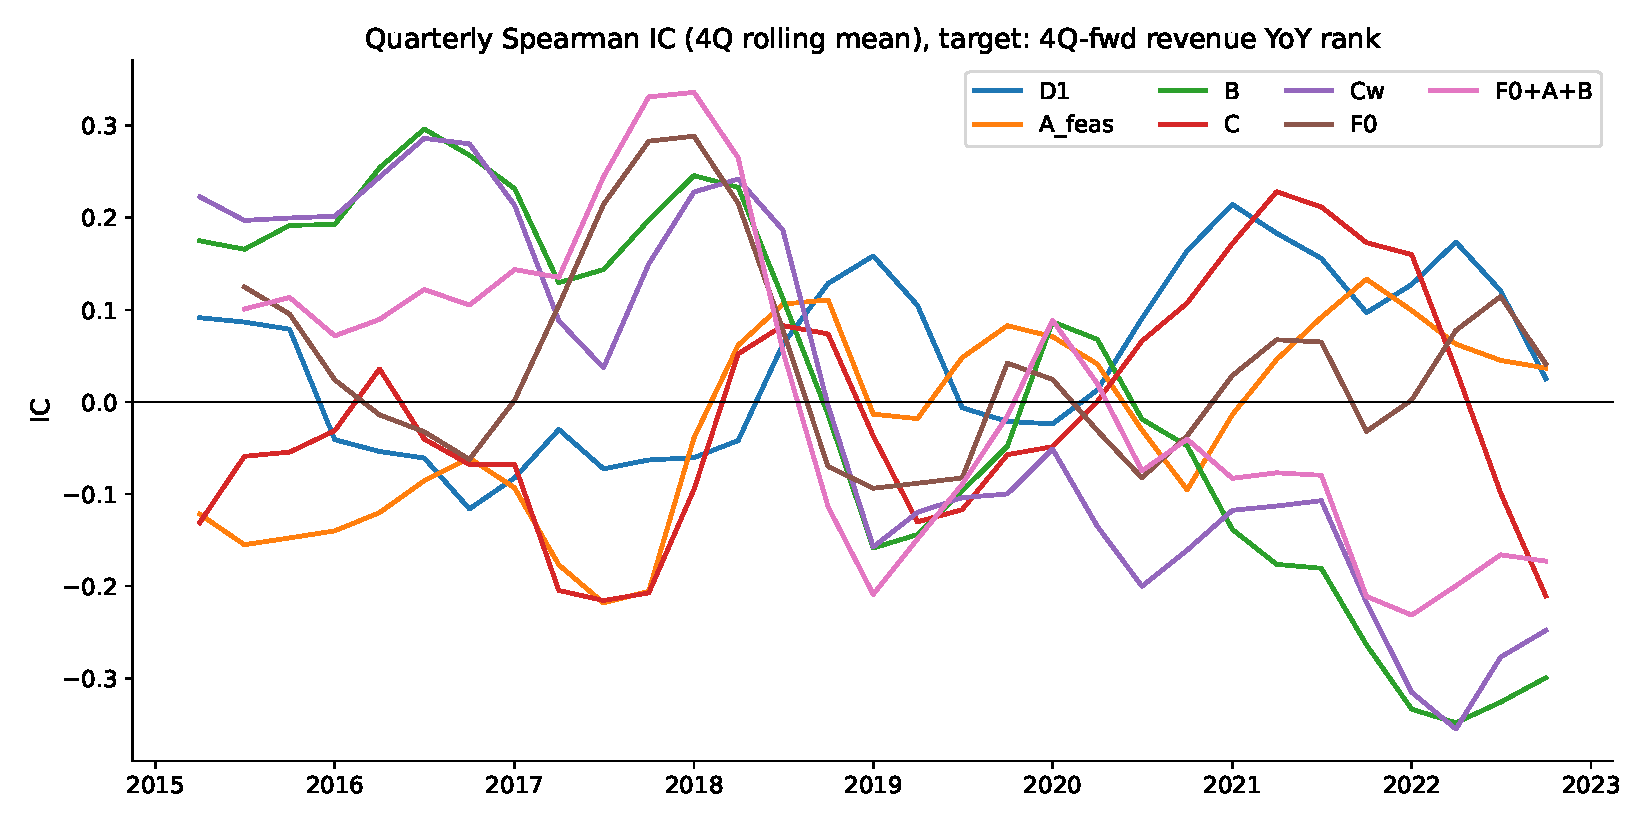
\includegraphics[width=0.92\linewidth]{fig09_ic_series.pdf}
  \caption{\textbf{Out-of-sample scoreboard: quarterly information coefficient.} Per-quarter cross-sectional Spearman IC (four-quarter rolling mean) against four-quarter-ahead revenue-growth rank, for the momentum baseline, the regime competitors, and the fundamentals combinations. No hidden-Markov feature consistently beats the simple baselines.}
  \label{fig:ic}
\end{figure}

The headline is the marginal contribution of patent-regime features over fundamentals, and it is zero. Adding the patent-only regime probability to a fundamentals baseline changes its information coefficient by $+0.002$ (Newey-West $t=0.23$); adding both patent and financial regime probabilities changes it by $-0.035$ ($t=-0.77$). Patent-rhythm regime features add no marginal predictive value for future revenue growth. We note, equally, that all signals are weak---the winning baselines themselves carry information coefficients below 0.04---which indicates that the target is only marginally predictable in this universe and period, and we are careful not to over-interpret a contest among weak predictors (Figure~\ref{fig:marginal}).

\begin{figure}[htbp]
  \centering
  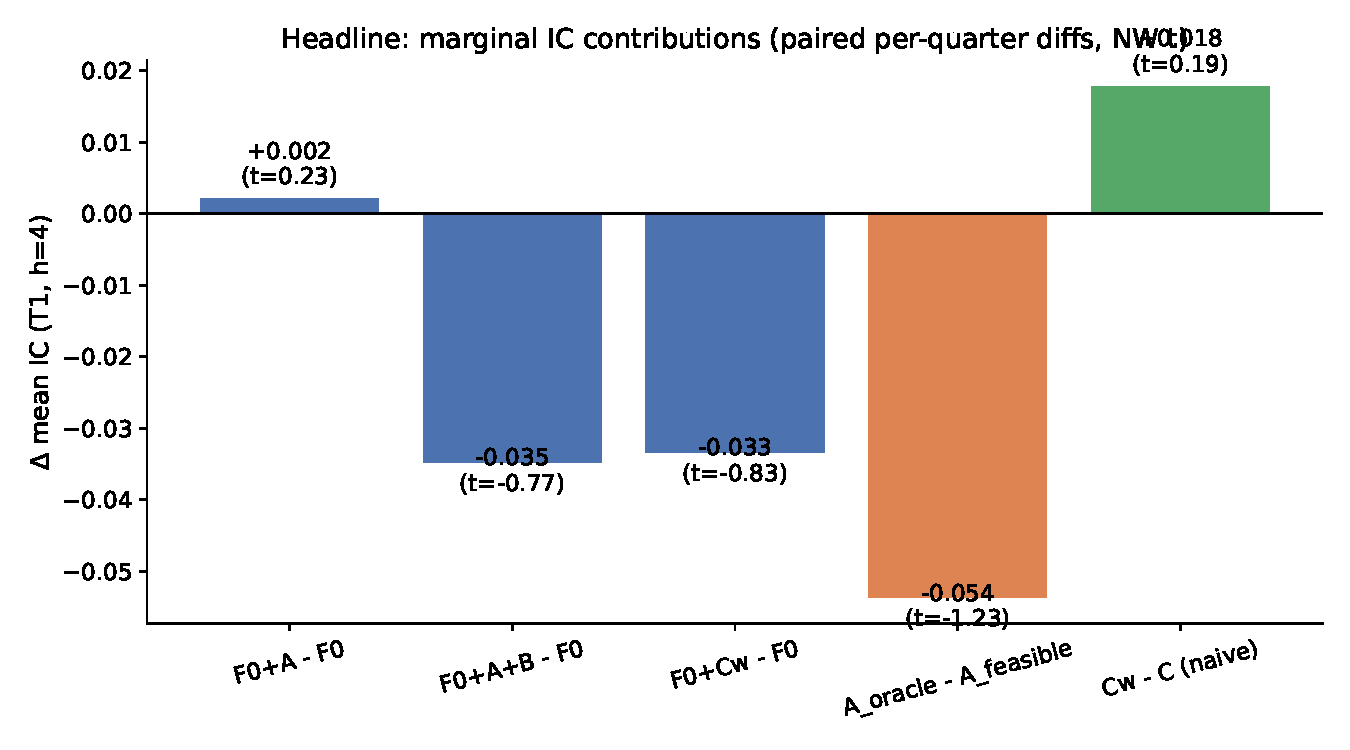
\includegraphics[width=0.7\linewidth]{fig10_marginal.pdf}
  \caption{\textbf{Headline: the marginal contribution of regime features is zero.} Change in mean IC (primary horizon) from adding each regime feature to the fundamentals baseline, as paired per-quarter differences with Newey-West $t$-statistics. Adding patent-regime features does not significantly improve on fundamentals.}
  \label{fig:marginal}
\end{figure}

\subsection{The publication lag is free, and calibration confirms the diagnosis}

Two secondary results sharpen the picture. First, the oracle does not beat the feasible series: the difference in information coefficient is $-0.054$ ($t=-1.23$), and the oracle patent feature is, if anything, significantly negative on its own ($-0.072$, $t=-2.58$). The eighteen-month publication lag is therefore \emph{costless} in predictive terms---not because the lag is harmless, but because the channel carries no forward-looking signal that being early would help exploit. This is our answer to the question of how the filing-publication-grant timing affects prediction: under a count-based signal, it does not.

Second, the tempered model independently confirms the scale diagnosis of Section~5. Selected by out-of-sample inner validation across the 32 windows, the weight on the Negative-Binomial term is suppressed to roughly 10\% in the large majority of windows---exactly the correction the scale argument predicts, arrived at here purely by predictive performance rather than by assumption. Yet calibration does not manufacture a signal: the tempered model's information coefficient exceeds the naive joint model's by only $+0.018$ ($t=0.19$), not significantly. Even well-calibrated fusion cannot compensate for the absence of signal in the underlying channel.

\subsection{The one significant relation, and what it is not}

A single relation in the scoreboard is statistically significant: the oracle patent-regime feature is negatively associated with subsequent revenue-growth rank. Because a negative result invites over-reading of any significant cell, we subjected it to a post-hoc robustness check, labeled as such. The negative relation is not a size artifact: residualizing the feature on firm size (log revenue) leaves the information coefficient essentially unchanged, indeed slightly stronger ($-0.072$ to $-0.084$, $t=-3.02$), and the feature is not absorbed when added to a fundamentals-plus-size combination (marginal $-0.024$, $t=-2.32$); a premise check confirms that size itself barely predicts growth rank in this universe, so size cannot mechanically explain the relation. We nonetheless decline to interpret this as a tradeable contrarian signal: it appears only in the infeasible oracle variant (the feasible marginal is $+0.003$, insignificant), it emerges from many comparisons, and the robustness check eliminates only the size confound, not alternative mechanical explanations such as firm age, maturity, or sub-sector composition. We flag it as an exploratory observation for future, separately pre-registered work, not as a finding of this paper.

\section{Discussion}

\subsection{Interpretation}

Our results answer the motivating question in the negative, but the negative is specific and bounded. We do not find that innovation is irrelevant to fundamentals, nor that patents contain no information; we find that the \emph{rhythm of patent counts}, modeled as a regime signal, adds no marginal predictive value for four-quarter-ahead revenue growth in this universe, over and above simple fundamentals, and that this holds across single-channel, naive-fusion, and calibrated-fusion specifications and under both feasible and oracle information. The most economical reading is that the count of patents is too crude a sensor of the latent quality state: it registers that a firm is active, and how active, but not whether that activity is the kind that translates into future growth. Micron, our control, makes the point concretely---it is among the most prolific patenters in the panel, yet its revenue is governed by a memory cycle the patent channel cannot see.

Two results survive this negative and stand on their own. The diagnosis that naive likelihood-based fusion weights channels by measurement scale rather than economic informativeness is, we believe, the paper's most transferable contribution: it is a general hazard for anyone fusing heterogeneous sensors---counts with continuous ratios, high-frequency with low-frequency series---in a single likelihood, and our out-of-sample finding that data-driven calibration independently drives the dominant channel to a tenth of its naive weight quantifies the distortion. Separately, the measurement that restatements roughly double the apparent strength of a momentum signal is a concrete caution for the broad practice of backtesting fundamental signals on as-currently-reported data.

\subsection{Limitations}

Several limitations bound our claims and, in turn, define what would be required to overturn them. Our universe is a single industry of 52 firms; the panel is wide enough for cross-sectional ranking but far from the breadth at which a weak signal might become reliably estimable, and a richer signal might require it. Our attrition is non-random in a way we cannot fully correct: acquisitions tend to follow good performance, so firms censored by delisting are not a random sample, which biases any in-sample relationship between regime state and subsequent outcomes. Our patent measure, despite careful entity resolution and reattribution, remains a count; we make no use of patent text, claims, citations, or classification beyond the firm match. And our target is revenue growth---chosen for its alignment with the ``technology becomes sales'' thesis---rather than margins, returns, or earnings, each of which would test a different link in the chain from innovation to value, and one of which (gross-margin change) shows a marginal patent contribution in an exploratory cell that we explicitly decline to over-read.

\subsection{What would be required: better sensors}

The framing that organizes both our method and our negative result also points to its sequel. If the count of patents is the crudest sensor of latent quality, the natural research program is to replace it with progressively more informative ones and to re-run the same disciplined, point-in-time, pre-registered evaluation. Three sensors are immediate candidates. \emph{Quality-weighted} patents---weighting by citations received, family size, or renewal behavior---would test whether the issue is patents per se or merely their undifferentiated counting. \emph{Citation-network} features---a firm's position in the directed graph of who cites whom---would capture technological centrality that raw counts ignore. Most promising, and most aligned with the domain, are \emph{standard-essential-patent} signals: a firm's position in the standardization of a technology has been linked to firm value \citep{hussinger2015,baron2016}, and recent work relates patent--standard proximity to firm growth \citep{bergeaud2022}. What remains open, to our knowledge, is the evaluation of such standard-position signals as \emph{forward-looking predictors of fundamentals within a pre-registered, point-in-time, out-of-sample framework} of the kind we develop here---rather than as contemporaneous or retrospective firm-level associations. Our contribution is to provide the evaluation harness within which such sensors can be tested honestly; this paper establishes the floor that any of them must clear.

\section{Conclusion}

We asked whether the rhythm of patent activity anticipates future fundamentals, and built a reproducible, survivorship-aware, point-in-time framework to answer it honestly. Within a pre-registered out-of-sample evaluation, the answer for a count-based patent signal is negative: patent-rhythm regime features add no marginal predictive value for four-quarter-ahead revenue growth over simple fundamentals, whether used alone, in naive fusion, or in calibrated fusion, and whether under a realistic publication lag or an infeasible oracle---while the simple baselines that beat them are themselves weak, indicating a target that is only marginally predictable here. The value of the exercise lies elsewhere: in a diagnosis that naive likelihood-based fusion weights channels by measurement scale rather than economic informativeness, confirmed out of sample by a calibration that independently suppresses the dominant channel to a tenth of its weight; in a quantification of how restatements inflate momentum backtests; and in establishing, through the discipline of pre-registration, a credible floor that richer innovation sensors---quality-weighted, citation-network, and standard-essential-patent signals---must clear. We see the count of patents as the crudest sensor of latent corporate quality, and this paper as the harness within which better sensors can be tested. That a carefully-built signal does not work, established under discipline that prevents us from pretending otherwise, is a more useful starting point for that program than a fragile positive would have been.

\bibliographystyle{plainnat}
\bibliography{references}

\appendix
\renewcommand{\thesection}{Appendix~\Alph{section}:}

\section{Data and Code Availability}

All data derive from two public sources---Google Patents Public Data (\texttt{patents-\allowbreak public-\allowbreak data.\allowbreak patents.\allowbreak publications}) on BigQuery and the SEC EDGAR XBRL \texttt{companyfacts} API---and all code, queries, the firm registry, the merger-reattribution table, and the pre-registration deviation log are available in the replication repository at \url{https://github.com/anilberkekarel/quality-engine-v2}. The universe definition, assignee-matching rules and exclusions, predecessor-CIK merges, and the QCOM amendment are recorded with timestamps preceding the predictive analysis.

\section{Deviation Log}

The pre-registration is the locked-constant block and protocol docstring of the scoreboard code; any change made after results existed is recorded here. Three deviations occurred, none of which altered feature sets, parameter grids, thresholds, targets, or the primary result.

\textbf{(a) AUC null correction.} The Newey-West $t$-statistic for the Tier-1 AUC metric (target T2, top-quintile classification) was initially computed against a null of 0; it was corrected post-run to test against the chance level of 0.5. This is a reporting fix to the significance of the AUC columns; it changes no IC result and no point estimate, only the $t$-statistics of the AUC rows.

\textbf{(b) Tempered-model inner validation and state ordering.} The tempered joint competitor (Cw) selects its Negative-Binomial down-weight $w$ per window by a fully causal nested inner validation---a mini-backtest scoring each candidate $w$ by the cross-sectional IC of the window-$s$ feature (filtered high-regime probability from the model fit on data up to $s$) against targets realized by $t$, over $s$ in $[\text{2011Q1},\, t-4]$. This procedure, together with the locked state-ordering convention (competitors A and C order their states by the patent-count mean, while B and Cw order by the gross-margin mean---because Cw's patent channel is down-weighted, a fully-weighted channel must define the ``high'' state), was clarified in writing and locked before the run.

\textbf{(c) Acquirer-side merger rows.} The merger-window $\pm$2-quarter exclusion robustness (Tier-1, $h=4$ ICs recomputed dropping company-quarters within two quarters of a firm's merger events) was extended by adding acquirer-side rows to the merger-events table, so that the exclusion covers both sides of each transaction rather than only the acquired side. This addition was made before the scored run.

\section{Supplementary Results}

This appendix reports the exploratory and robustness results referenced in the main text. All numbers are read directly from the replication output CSVs (\texttt{scoreboard.csv} and \texttt{scoreboard\_\allowbreak size\_\allowbreak robustness.\allowbreak csv}). Tier-1 rows are single features; Tier-2 rows are expanding-window combiners; F0 denotes the fundamentals combination.

\begin{table}[htbp]
  \centering
  \caption{Gross-margin-change target (T3): universe-median-adjusted gross-margin change at $t+4$, scored by cross-sectional Spearman IC with Newey-West $t$. The exploratory cell noted in the main text is the marginal patent contribution F0+A over F0.}
  \label{tab:t3}
  \begin{tabular}{lrrr}
    \toprule
    Competitor & IC & NW $t$ & $n$ \\
    \midrule
    D1 (revenue momentum) & $-0.039$ & $-1.11$ & 32 \\
    D2 (prior-year quintile) & $-0.035$ & $-1.01$ & 32 \\
    A feasible (patent-only) & $-0.012$ & $-0.36$ & 32 \\
    A oracle (patent-only) & $-0.042$ & $-0.89$ & 32 \\
    B (financial-only) & $-0.065$ & $-0.89$ & 32 \\
    C (naive joint) & $-0.016$ & $-0.47$ & 32 \\
    Cw (tempered joint) & $-0.055$ & $-0.95$ & 32 \\
    \midrule
    F0 (fundamentals) & $+0.132$ & $+1.98$ & 31 \\
    F0+A & $+0.143$ & $+2.28$ & 31 \\
    F0+B & $+0.096$ & $+1.52$ & 31 \\
    F0+A+B & $+0.114$ & $+2.05$ & 31 \\
    F0+Cw & $+0.112$ & $+1.83$ & 31 \\
    \bottomrule
  \end{tabular}
\end{table}

\begin{table}[htbp]
  \centering
  \caption{Net-income-direction target (appendix to T2): direction of NetIncomeLoss change at $t+4$ versus $t$, scored by AUC with Newey-West $t$ against the 0.5 null. No competitor shows signal (all AUC $\leq 0.49$).}
  \label{tab:nidir}
  \begin{tabular}{lrrr}
    \toprule
    Competitor & AUC & NW $t$ & $n$ \\
    \midrule
    D1 (revenue momentum) & 0.479 & $-0.85$ & 31 \\
    D2 (prior-year quintile) & 0.478 & $-0.92$ & 31 \\
    A feasible (patent-only) & 0.492 & $-0.34$ & 31 \\
    A oracle (patent-only) & 0.460 & $-1.63$ & 31 \\
    B (financial-only) & 0.464 & $-1.43$ & 31 \\
    C (naive joint) & 0.456 & $-1.57$ & 31 \\
    Cw (tempered joint) & 0.485 & $-0.78$ & 31 \\
    \bottomrule
  \end{tabular}
\end{table}

\begin{table}[htbp]
  \centering
  \caption{Merger-window $\pm$2-quarter exclusion robustness: primary-horizon ($h=4$) IC with all company-quarters versus excluding those within two quarters of a firm's merger events. The ranking is unchanged by the exclusion.}
  \label{tab:maexcl}
  \begin{tabular}{lrr}
    \toprule
    Competitor & IC (all) & IC (M\&A-excl.) \\
    \midrule
    D1 (revenue momentum) & $+0.037$ & $+0.047$ \\
    D2 (prior-year quintile) & $+0.039$ & $+0.046$ \\
    A feasible (patent-only) & $-0.018$ & $-0.013$ \\
    A oracle (patent-only) & $-0.072$ & $-0.057$ \\
    B (financial-only) & $-0.002$ & $+0.010$ \\
    C (naive joint) & $-0.030$ & $-0.009$ \\
    Cw (tempered joint) & $-0.013$ & $+0.016$ \\
    \midrule
    F0 (fundamentals) & $+0.031$ & $+0.052$ \\
    F0+A & $+0.033$ & $+0.046$ \\
    F0+B & $-0.009$ & $+0.004$ \\
    F0+A+B & $-0.004$ & $+0.003$ \\
    F0+Cw & $-0.003$ & $+0.025$ \\
    \bottomrule
  \end{tabular}
\end{table}

\begin{table}[htbp]
  \centering
  \caption{Latest versus as-filed target: primary-horizon ($h=4$) IC scored against the as-filed (point-in-time) target versus the most-recently-restated (latest) target. The momentum baselines roughly double on restated data---the restatement-inflation finding of Section~3.4.}
  \label{tab:latest}
  \begin{tabular}{lrrr}
    \toprule
    Competitor & IC (as-filed) & IC (latest) & ratio \\
    \midrule
    D1 (revenue momentum) & $+0.037$ & $+0.079$ & 2.14 \\
    D2 (prior-year quintile) & $+0.039$ & $+0.081$ & 2.09 \\
    A feasible (patent-only) & $-0.018$ & $-0.020$ & --- \\
    A oracle (patent-only) & $-0.072$ & $-0.063$ & --- \\
    B (financial-only) & $-0.002$ & $-0.028$ & --- \\
    C (naive joint) & $-0.030$ & $-0.028$ & --- \\
    Cw (tempered joint) & $-0.013$ & $-0.039$ & --- \\
    \bottomrule
  \end{tabular}
\end{table}

\begin{table}[htbp]
  \centering
  \caption{Size-confound robustness (post-hoc, not pre-registered) for the A oracle negative IC of Section~6.4. Size $=\log(\text{revenue})$, same point-in-time rule as the baseline features. Panel A: size barely predicts growth, though it correlates weakly with the patent feature. Panel B: residualizing on size leaves the A-feature IC essentially unchanged (raw shown with NW $t$ in parentheses). Panel C: the patent feature is not absorbed by a fundamentals-plus-size combiner (F0s).}
  \label{tab:size}
  \begin{tabular}{lrr}
    \toprule
    \multicolumn{3}{l}{\emph{Panel A: diagnostics}} \\
    & estimate & NW $t$ \\
    \midrule
    size $\to$ growth, $h=4$ (IC) & $-0.026$ & $-0.51$ \\
    size $\to$ growth, $h=8$ (IC) & $+0.045$ & $+0.81$ \\
    corr(A oracle, size) ($\rho$) & $+0.153$ & $+3.48$ \\
    corr(A feasible, size) ($\rho$) & $+0.122$ & $+3.13$ \\
    \midrule
    \multicolumn{3}{l}{\emph{Panel B: raw vs.\ size-residualized A feature (IC, NW $t$)}} \\
    & raw & size-residualized \\
    \midrule
    A oracle, $h=4$ & $-0.072$ ($-2.58$) & $-0.084$ ($-3.02$) \\
    A oracle, $h=8$ & $-0.065$ ($-1.87$) & $-0.065$ ($-1.94$) \\
    A feasible, $h=4$ & $-0.018$ ($-0.53$) & $-0.016$ ($-0.42$) \\
    A feasible, $h=8$ & $-0.054$ ($-1.38$) & $-0.065$ ($-1.44$) \\
    \midrule
    \multicolumn{3}{l}{\emph{Panel C: Tier-2 marginal over fundamentals+size, $h=4$}} \\
    & $\Delta$IC & NW $t$ \\
    \midrule
    F0s+A feasible $-$ F0s & $+0.003$ & $+0.34$ \\
    F0s+A oracle $-$ F0s & $-0.024$ & $-2.32$ \\
    F0s $-$ F0 & $+0.018$ & $+0.24$ \\
    \bottomrule
  \end{tabular}
\end{table}

\end{document}
